\chapter{资金的等值计算}
\section{资金的时间价值(注重理解)}
资金的价值既体现在额度上,同时也体现在发生的时间上。不同时间发生的等额资金在价值上的差别,就称为资金的\textbf{时间价值}。

\textbf{引例1:}C公司年初从Y银行借入1000万元,并约定借期为N年,贷款年利率为6\% ;

(1)从C公司角度看,借用他人的资源,是要付出代价的,即利息,并且时间越长,付出的代价(成本、费用)越多。(与I和N都有关系)。

(2)从Y银行角度看,经营借贷业务的主要目的是通过利息赢利。并且时间越长,增值(赢利)越多。

\textbf{引例2:}现在的500万元,与将来(5年后)的500万元,在价值上不等。那么,现在的500万元,与将来(5年后)的多少万元,在价值上相等?(年利率12\%)。

资金随着时间的推移,会产生价值的变化——增值。

时间越长,资金的增值越多。表现为:利息多了、利润多了等等。

计量增值的方法可以用总利息或利润的多少来计量,也可以用单位时间的利息或利润的多少来计量,即用利率来计量。反时间方向来认识这一现象,就是“将来时间上的一笔数额的资金,在现在看来是不值那么多的”。

\textbf{资金具有时间价值的内涵:}

资金在生产与交换过程中由于有劳动者的劳动使之产生了增值。资金的时间价值是对放弃现时消费的必要补偿。

\subsection{影响资金使用的因素}

\begin{itemize}
    \item 投资收益率
    \item 风险
    \item 通货膨胀
\end{itemize}

\subsection{概念}
不同时间发生的等额资金在价值上的差别称为资金的时间价值。也即资金在生产和流通过程中随着时间推移而产生的增值。

对资金使用者来讲,是使用资金的成本。

如:某项目投资100万元,建成投产后,每年可得利润20万元,即为100万元在特定生产经营活动中所产生的时间价值。

\subsection{涵义}
(1)资金随着时间的推移,其价值会增加。

(2)从消费者角度讲,是对放弃现期消费的补偿。

\subsection{资金时间价值表现形式}
一是资金投入生产或流通领域产生的增值称为利润(Profit)或收益(Income);

二是把资金存入银行或向银行借贷所得到或付出的增值额称为利息(Interest)。

\subsection{资金时间价值衡量尺度}
(1)绝对尺度:体现资金时间价值绝对量的多少。利息、利润或收益;

(2)相对尺度:反映资金时间价值相对量的大小。利息率、利润率或收益率。

\subsection{资金时间价值的意义}
项目的经济评价中,必须增强资金的时间观念,用动态的观点看待资金的使用,考虑资金的时间价值,采用动态分析方法将不同的费用或效益折算成同一时点来进行比较。

\subsection{资金等值的概念}

资金等值是指在不同时点绝对值不等而价值相等的资金。

在一个或几个项目中,投资或收益往往发生在不同的时间,于是就必须按照一定的利率将这些投资或收益折算到某一个相同的时点,这一过程就是等值计算。

\section{利息和利率}
\subsection{利息$I_n$}
贷款人向借款人让渡资金使用权而得到的一种报酬,也是借款人占用资金所付的代价。

某人存入银行一笔资金,存期\textbf{5年}(\textbf{计息期}),\textbf{每年}(\textbf{计息周期(每次计算利息的时间单位)})计息一次,整个存储期间共计息\textbf{5次}(\textbf{n:计息周期次数})。

\subsection{利息的表示方式}
\subsubsection{(1)绝对数表示:}
$$I_n = F_n - P$$
$F_n$:经过$n$个计息周期后的本利和。
\subsubsection{(2)相对数表示:}
指单位本金经过一个计息周期的利息数额。
$$i = \frac{I_1}{P} \times 100\%$$

\subsection{利率i}

一定时期内(一年、半年、月、季度,即一个计息周期)利息总额与本金(借贷金额)的比率。

$$\mbox{利率} = \frac{\mbox{期利息}(I_1)}{\mbox{本金}(P)} \times 100\%$$

利率是单位本金经过一个计息周期后的增殖额。(年利率、半年利率、月利率,……)

\subsection{利息计算方法}
\subsubsection{(1)单利法}

仅对本金计息,利息不再生利息。
$$I_n= p \cdot n\cdot i$$
$$F_n=P \cdot (1+i \cdot n)$$

P为本金,n为计息期数(通常为年),i代表利率,I代表所付或所收的总利息,F代表本利和。

\begin{figure}[H]
    \centering
    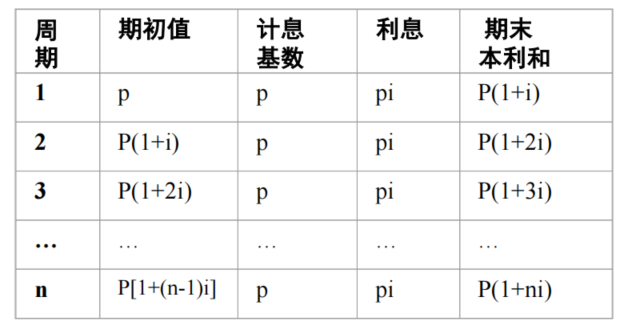
\includegraphics[width=0.9\linewidth]{image/单利法本利和公式推导.png}
    \caption{单利法本利和公式推导}
\end{figure}

\subsubsection{(2)复利法}

核心:以本金与累计利息之和为计息基数,即“利上加利”、“利滚利”、“驴打滚”。

技术经济分析中时间价值一般采用复利法,充分反映资金的时间价值。

\begin{figure}[H]
    \centering
    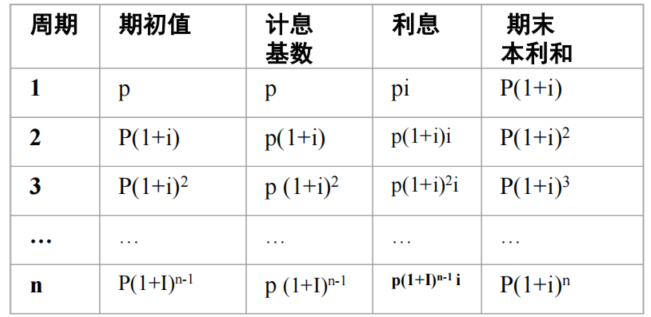
\includegraphics[width=0.9\linewidth]{image/复利法本利和公式推导.png}
    \caption{复利法本利和公式推导}
\end{figure}

$$F_n=P \cdot (1+i)^n$$

\begin{itemize}
    \item $P$:原始本金;
    \item $i$:一个计息周期利率;
    \item $n$:计息期内计息周期次数。
\end{itemize}

\subsubsection{(3)差异分析}
单利计息:对资金时间价值的考虑不完整,利息没转入记息基数;

复利计息:充分反映资金的时间价值。


\subsection{名义利率和实际利率}
\subsubsection{(1)名义利率}
在技术经济分析中,复利计算通常以年为计息周期。但在实际经济活动中,计息周期有年、半年、季、月等多种,这样出现了不同计息周期的利率换算问题。

如:按月计算利息,且其月利率为1\%,通常称为“年利率12\%,每月计息一次”。这个年利率12\%称为“\textbf{名义利率}”。

名义利率的计算:
$$\mbox{名义利率}(r) = \mbox{每一计息周期的利率} \times \mbox{一年中的计息周期的次数}(m)$$
$$r/m = \mbox{每一计息周期利率}$$

\subsubsection{(2)实际利率}
\textbf{实际利率:}当一年内多次复利计息时,按照一年内获得的利息与年初本金之比计算出的年利率为实际年利率。

实际利率的计算:
$$\mbox{实际利率}(i)=\mbox{一年内按复利计息的利息总额}/\mbox{年初本金}$$\\
举例:
本金1000元,每月复利计息一次,月利率1\%,一年后的本利和为:
$$F = 1000 \times (1+1\%)^{12}= 1126.8 \mbox{(元)}$$
实际利率为:
$$\frac{1126.8-1000}{1000} \times 100\%=12.68\%$$

\subsubsection{(3)名义利率和实际利率公式推导(我认为不需要掌握,但是看两眼)}
复利计息,一年后本利和为:
$$F=P(1+r/m)^m$$

一年内的利息额为:
$$I=F-P=P \times (1+r/m)^m-P=P \times [(1+r/m)^m-1]$$

实际利率为:
$$i=(F-P)/P=\frac{P \times (1+r/m)^m-p}{p}=(1+r/m)^m-1$$

若计息周期为一年,$m = 1$,则$i = r$,即实际利率=名义利率。

若连续计息, $m \to \infty$,则:
$$i = \lim_{m \to \infty}(1+\frac{r}{m})^m-1=e^r-1$$

若名义年利率为12\%,以下各种情况下,实际年利率等于多少?

\textcircled{1}按年计息,m=1
$$i = (1+ r/m)^m-1=(1+0.12/1)^1-1=12\%$$

\textcircled{2}按半年计息,m=2
$$i = (1+ r/m)^m-1=(1+0.12/2)^2-1=12.36\%$$

\textcircled{3}按季度计息,m=4
$$i = (1+ r/m)^m-1=(1+0.12/4)^4-1=12.55\%$$

\textcircled{4}按月计息,m=12
$$i = (1+ r/m)^m-1=(1+0.12/12)^{12}-1=12.68\%$$

\textcircled{5}按连续计息,m=$\infty$
$$i=e^r-1=e^{0.12}-1=12.75\%$$
\textbf{例1:}某人将1000元存入银行,定期3年,年利率12\%,3年期满,按复利计算,期满后他可以从银行得到[填空1]元。\\
\textbf{答案:}\\
实际利率:$i=(1+\frac{12\%}{12})^{12}-1=1.01^{12}-1=12.68\%$\\
应归还本利和:$20 \times (1+12.68\%)^3=20 \times 1.4308=28.62$(万元)\\
\textbf{例2:}下列说法正确的是\\
A. 名义年利率条件下,一年的利息额是按单利计算
\\
B. 实际年利率条件下,一年的利息额是按单利计算
\\
C. 实际年利率条件下,一年的利息额是按复利计算
\\
D. 名义年利率条件下,一年的利息额是按复利计算\\
\textbf{答案:}AC\\
\textbf{例3:}(判断题)若一年中复利计息的次数大于1,则年实际利率小于年名义利率。\\
\textbf{答案:}错误\\
差异原因分析:
$$\mbox{年利率}i=\frac{\mbox{一年的利息额}}{\mbox{年初本金}} \times 100\%$$
名义年利率:一年的利息额是按单利计算的;\\
实际年利率:一年的利息额是按复利计算的;\\
当一年中多次计息时(即$m>1$时),两者产生差异。


\section{资金的等值计算}

\subsection{基本概念}

资金的时间价值:在不同的时间付出或得到同样数额的资金在价值上是不等的,即资金的价值会随着时间发生变化。

评价技术的经济效果,不仅要考虑现金流入、流出的数额,还要考虑每笔现金流量发生的时间。

不同时间发生的等额资金在价值上的差别称为资金的时间价值。也即资金在生产和流通过程中随着时间推移而产生的增值。对资金使用者来讲,是使用资金的成本。

某项目投资100万元,建成投产后,每年可得利润20万元,即为100万元在特定生产经营活动中所产生的时间价值。

\subsubsection{决定资金等值的因素}
\begin{itemize}
    \item 资金数额
    \item 资金发生的时刻
    \item 利率:关键因素
\end{itemize}

资金随着时间的推移,其价值会增加。从消费者角度讲,是对放弃现期消费的补偿。

\subsubsection{资金的时间价值引发的问题}

\begin{figure}[H]
    \centering
    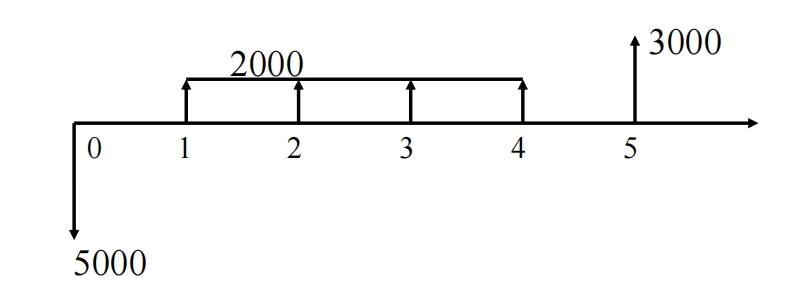
\includegraphics[width=0.8\textwidth]{image/资金时间价值引发的问题.png}
    \caption{资金时间价值引发的问题}
    \label{fig:3}
\end{figure}

不能直接比较不同时间点的资金的价值大小;

需要利用等值换算,将不同时点的资金换算到同一时点进行比较。

\subsubsection{资金时间价值表现形式}
\begin{itemize}
    \item 资金投入生产或流通领域产生的增值称为利润(Profit)或收益(Income)。
    \item 把资金存入银行或向银行借贷所得到或付出的增值额称为利息(Interest)。
\end{itemize}

\subsubsection{资金时间价值衡量尺度}
(1)绝对尺度:体现资金时间价值绝对量的多少。利息、利润或收益;

(2)相对尺度:反映资金时间价值相对量的大小。利息率、利润率或收益率。

\subsection{资金等值}
\subsubsection{概念}
在考虑资金时间价值的情况下,在不同的时间绝对值数额不等的若干资金,如果具有相同的价值,则为等值的资金。

例如,年初的100元和年底的110元,在单利10\%的情况下是等值的。

\subsubsection{资金等值概念的意义}
利用等值概念,通过等值计算,可以知道某一时点上的资金金额在其他时点上的价值。可以把不同时点发生的资金金额换算到同一时点进行价值比较。
\subsubsection{相关概念}
等值资金:在利率一定的条件下,我们把不同时间(时期、时点)上绝对数额不等,而经济价值相等的若干资金,称为等值资金。

资金等值计算:利用资金等值原理,我们可以把某一时间点上的资金值,按照所给定的利率换算为与之等值的另一时间点的资金值,这一换算过程称为资金的等值计算。

折现(贴现Discount):把将来某一时间点上的资金值换算成现在时间点上的等值资金值。

折现率($i$,Discount Rate):进行资金等值计算中使用的反映资金时间价值的参数叫折现率。(如利率、收益率)

现值($P$,Present Value):“现值”并非专指一笔资金“现在”的价值,它是一个相对的概念。一般地说,将$t+k$个时点上发生的资金折现到第$t$个时点,所得的等值金额就是$t+k$个时点上的资金金额的现值。

终值($F$,Future Value):与现值等价的将来某时点的资金值称为“终值”。

等年值($A$,年金,Annual Value):分期等额收支的资金值。\\
\textbf{例题:}(判断)折现是指将来时点的资金金额换算成期初时点的资金金额这一过程。\\
\textbf{答案:}错误。

\section{资金等值计算公式(重点掌握)}
按照现金流的不同,等值公式可以分为:

一次收付类型:两个

等额分付类型:四个(另引申四个)

等差序列类型(自学,了解)

等比序列类型(自学,了解)

\subsection{一次收付型}
是指所分析系统的现金流量,无论是流入还是流出,均在一个时间点上一次发生。包括:

一次收付终值(未来值)公式

一次收付现值公式

\subsubsection{一次收付终值公式($P \to F$)}

\begin{figure}[H]
    \centering
    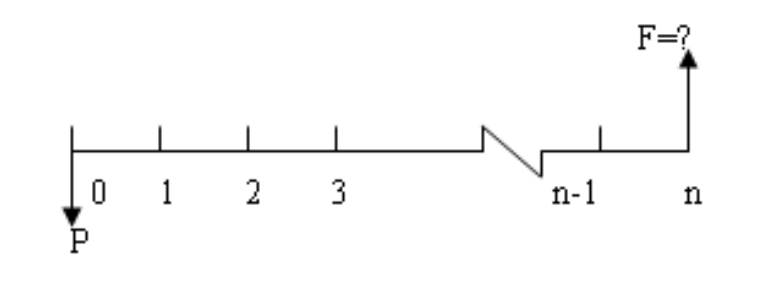
\includegraphics[width=0.8\textwidth]{image/一次收付终值现金流量图.png}
    \caption{一次收付终值现金流量图}
    \label{fig:3}
\end{figure}

已知$P$,求$F$,即求$P$在$n$年后的等值资金$F$

复利终值计算公式:\\
(与复利计息本利和计算公式相同)
$$F=P \cdot (1+i)^n$$

或

$$F=P \cdot (F/P,i,n)$$



\textbf{整付终值计算公式}

已知期初投资为$P$,利率为$i$,求第n年末收回本利$F$。
$$F=P(1+i)^n$$

$(1+i)^n$称为整付终值系数,记为$(F/P,i,n)$。

$(F/P,i,n)$中,$F$为欲求因素,其余为已知因素。复利终值系数可查表,如图\ref{fig:5}:

\begin{figure}[H]
    \centering
    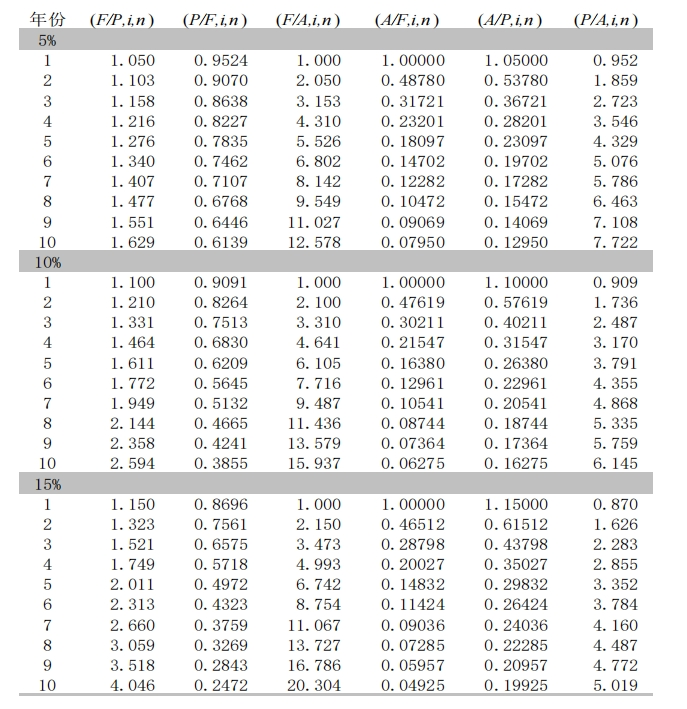
\includegraphics[width=\textwidth]{image/复利终值系数表.png}
    \caption{复利终值系数表}
    \label{fig:5}
\end{figure}

\subsubsection{一次收付现值公式($F \to P$)}
即在已知利率$i$的条件下,要想在$n$期期末得到资金$F$,期初应一次投入多少资金?其现金流量图如图\ref{fig:6}所示。

\begin{figure}[H]
    \centering
    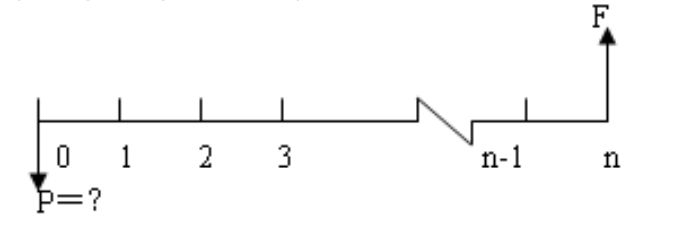
\includegraphics[width=0.8\textwidth]{image/一次收付现值现金流量图.png}
    \caption{一次收付现值现金流量图}
    \label{fig:6}
\end{figure}

\textbf{复利现值计算公式}
$$P=\frac{F}{(1+i)^n}=F \cdot (1+i)^{-n}$$(一次支付终值公式的逆运算)\\
或
$$P=F \cdot (P/F,i,n)$$(复利现值系数与复利终值系数互为倒数)\\
\textbf{例1:}给你一次选择机会,你可以现在获得1000元,也可以在5年以后的今天获得1300元,在年利率为8\%的情况下,你将做何种选择?\\
\textbf{答案:}$P=F/(1+0.08)^5=1300/(1+0.08)^5=884.76$\\
由于在年利率为8\%时, 5年后的1300元等值于现在的884.76元,小于同一时点的1000元,故应该选择现在获得1000元。\\
\textbf{例2:}某人把1000元存入银行,设年利率为6\%,复利计息,5年后全部提出,共可得多少元?

$F=P(1+i)^n=1000 \times (F/P,6\%,5)=1000 \times 1.338=1338$(元)\\
\textbf{例3:}某环保制造企业计划建造一条生产线,预计5年后需要资金1000万元,设年利率为10\%,复利计息,问现需要存入银行多少资金?

$P=F(1+i)^{-n}=1000 \times (P/F,10\%,5)=1000 \times 0.6209=620.9$(万元)

\subsection{等额分付系列公式}

含义:
等额分付是多次支付形式的一种,多次支付指现金流入和流出在多个时点上发生,而不是集中在某个时点上。当现金流序列是连续的,且数额相等,则称为等额系列现金流。
\begin{itemize}
    \item 等额分付年金终值公式
    \item 等额分付偿债基金公式
    \item 等额分付年金现值公式
    \item 等额分付资本回收公式
\end{itemize}

\subsubsection{等额收付年金终值公式($A \to F$)}

若每期期末支付同等数额的资金$A$,在利率为$i$的情况下,$n$期后的未来值应该是多少?其现金流量图如图\ref{fig:7}所示。

\begin{figure}[H]
    \centering
    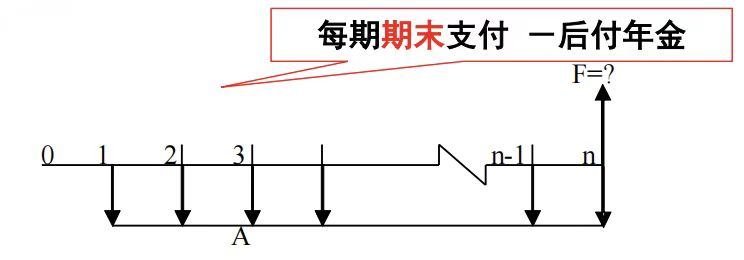
\includegraphics[width=0.8\textwidth]{image/等额收付终值现金流量图.jpg}
    \caption{等额收付终值现金流量图}
    \label{fig:7}
\end{figure}

\noindent \textbf{年金终值公式:}
$$F=A(1+i)^{n-1}+A(1+i)^{n-2}+\mbox{…}+A(1+i)+A=A \sum_{i=1}^{n} (1+i)^{n-1}=A[\frac{(1+i)^n-1}{i}]$$(利用等比级数求和公式)\\
或
$$F = A(F / A, i, n)$$(年金终值系数)\\
\textbf{例题:}某人从现在开始的三年内每年年末存入银行1000元,存款利率为10\%,复利计息,计算第三年年末该人银行账户的余额。\\
\textbf{答案:}$F=A \cdot (F/A,10\%,3)=1000 \times 3.310 = 3310$(元)\\
\textbf{引申:}如果上例改为“三年内每年年初存入银行1000元”,其他条件不变,则第三年年末该人银行账户的余额为多少?\\
\textbf{答案:}$F_d=A(F/A,10\%,3) \times (1+i)=1000 \times 3.310 \times (1+10\%)=3641$(元)

\noindent \textbf{先付年金}

$$F_d= A \cdot ( F / A , i , n ) \cdot (1 + i)$$

\begin{figure}[H]
    \centering
    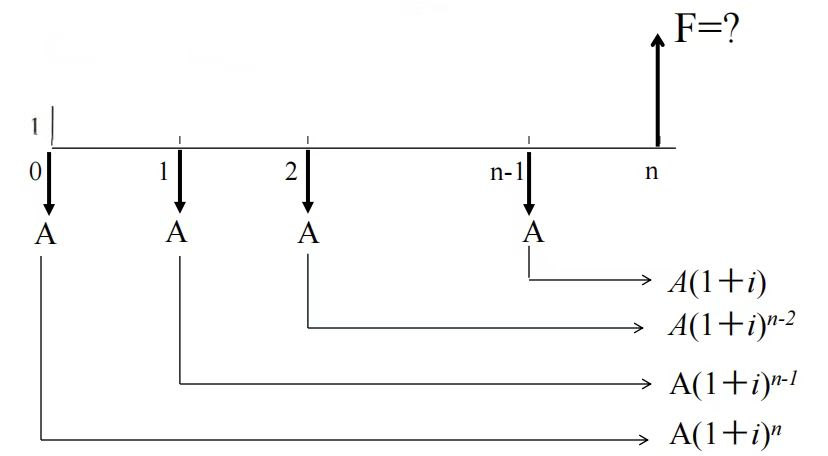
\includegraphics[width=0.8\textwidth]{image/先付年金图示.jpg}
    \caption{先付年金图示}
    \label{fig:8}
\end{figure}

\subsubsection{等额分付偿债基金公式($F \to A$)}
等额收付偿债基金公式是等额分付终值公式的逆运算。即已知终值F,求与之等值的等额年金A。\\
\textbf{偿债基金公式:}
$$A=F[\frac{i}{(1+i)^n-1}]$$
\textbf{偿债基金系数:}
$$A = F ( A / F , i , n )$$
\textbf{例题:}某人5年后需要10万元,他准备从现在起每年年末向银行存入一笔等额金额,已知存款年利率为5\%,复利计息,问每年的等额存款是多少?\\
\textbf{答案:}$A=100000(A/F,5\%,5)=100000 \times 0.18097)=18097$(元)\\
\textbf{引申:}如果上例改为每年年初向银行存入一笔等额金额,则每年的等额存款是多少?(提示:先付年金终值公式的逆运算)\\
\textbf{答案:}$A=100000(A/F,5\%,5)/(1 + 5\%)= (100000 \times 0.18097)/1.05= 17235$(元)

\subsubsection{等额分付年金现值公式$(A \to P)$}
若在每年年末等额分付资金$A$,在利率为$i$的条件下与之经济等值的现值为多少?其现金流量图\ref{fig:9}如图所示。

\begin{figure}[H]
    \centering
    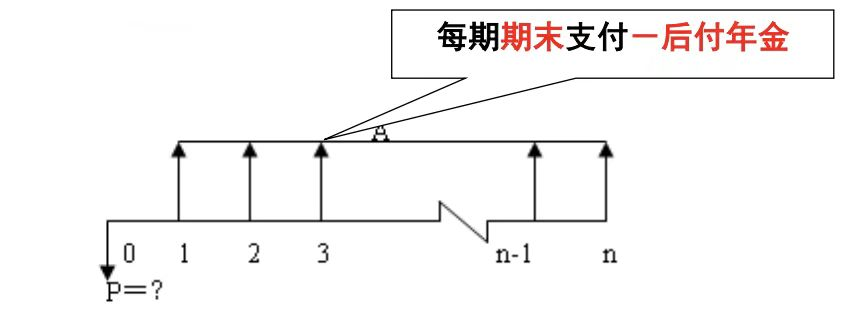
\includegraphics[width=0.8\textwidth]{image/等额收付现值现金流量图.jpg}
    \caption{等额收付现值现金流量图}
    \label{fig:9}
\end{figure}

\noindent \textbf{年金现值公式:}
$$P=A[\frac{(1+i)^n-1}{i(1+i)^n}]$$

\noindent \textbf{年金现值系数:}
$$P=A(P/A,i,n)$$

\noindent \textbf{例题:}某人为了在以后3年内每年年末可以从银行提取1000元,假设存款年利率为10\%,复利计息,问该人现在应该存入多少钱?\\
\textbf{答案:}$P=A(P/A,10\%,3)=1000 \times 2.487=2487$(元)\\
\textbf{引申:}上例中,如果改为“为了在以后3年内每年年初可以从提取1000元”,其他条件不变,则该人现在应该存入多少钱?\\
\textbf{答案:}$P_d=A \cdot (P/A,10\%,3) \cdot (1+i) =1000 \times 2.487 \times (1+10\%)=2735.7$(元)

\noindent \textbf{先付年金现值公式}
$$P_d=A[\frac{(1+i)^n-1}{i(1+i)^n}](1+i)$$
$$P_d=A(P/A,i,n)(1+i)$$

\noindent \textbf{特例——永续年金现值公式}
$$P=\frac{A}{1+i}+\frac{A}{(1+i)^2}+...\frac{A}{(1+i)^n}+...=A\lim_{n \to \infty}[\frac{(1+i)^n-1}{i(1+i)^n}]=\frac{A}{i}$$

\subsubsection{资本回收公式($P \to A$)}
资本回收公式是年金现值公式的逆运算,即已知现值$P$,求与之等值的年金$A$。

$$A=P[\frac{i(1+i)^n}{(1+i)^n-1}]$$

\noindent \textbf{资本回收系数:}
$$A=P(A/P,i,n)$$
\textbf{例题:}某人以分期付款的方式买下一套价值20万元的房子,年利率为8\%,付款期限为15年,每年付款额相等,问此人每年年末需要付多少钱?\\
\textbf{答案:}$A=200000(A/P,8\%,15)=200000 \times 0.11683=23367$(元)\\
\textbf{引申:}在上例中,如问此人每年年初需要付多少钱?(提示:先付年金现值公式的逆运算)\\
\textbf{答案:}$A=200000(A/P,8\%,15)/(1+i)=(200000 \times 0.11683)/(1+8\%)=21636$(元)

\section{本章思考题(必做)}
\noindent \textbf{思考题1:}某人连续10年每年年初存入银行1000元,名义利率10\%,半年复利计息一次,计算10年末此人存款的本利和是多少?

\noindent \textbf{思考题2:}2、假定第一年年初你存入银行10万元,年利率5\%,从第4年年末开始连续6年每年年末从银行取出相等的金额,使得存款账户余额为0。问每年取出的金额是多少?

\noindent \textbf{思考题3:}在你出生时,你的父母决定在你的每一个生日为你存款1000元,直到18岁。但是你的父母在你7岁和11岁时没有存款,假设年利率为5\%,当你18岁时,银行账户的余额是多少?

\noindent \textbf{思考题4:}某人与保险公司订立了一份养老保险合同。合同规定此人现在支付保险公司100,000元,在此后的15年中保险公司每年末付给他10,000元,问保险公司提供的年利率是多少?(给出利率区间即可)

\noindent \textbf{思考题5:}某人希望拥有100,000元的存款,为了实现这一目标,他计划从现在开始每年年初存入5,000元,年利率为8\%,问需要多少年?

\noindent \textbf{思考题6:}若年利率为13\%,连续n期期初年金的现值为46.38元,则连续n期期末年金的现值为多少?